\section{Resultados para o controlador por \textit{negative feedback}}

O controlador escolhido para apresentar os resultados práticos foi aquele projeto pelo método frequencial. 

\subsection{Projeto dos circuitos}

\subsubsection{Planta}

O circuito proposto para a planta da figura \ref{ckt:planta} foi obtido a partir de módulos propostos por KUO (1995).

\begin{figure}[H]
\begin{center}
\tikz \node [scale=0.70, inner sep=0] {
\begin{tikzpicture} [ american, ]
    \draw (0,0) node[op amp] (opamp1) {}
    (opamp1.+) -- (-1.5,-0.5) node[ground]{}
    (opamp1.-) to[R, l_=$R_3$, -*] (-4,0.5) 
    (opamp1.out) 
    ;
    \draw (6,-0.5) node[op amp] (opamp2) {}
    (opamp2.+) -- (4.5,-1) node[ground]{}
    (opamp2.-)  to[R, l_=$R_1$]  (opamp1.out)
    (opamp2.out) to[short, -*] (8,-0.5)
    ;
    \draw (-4.5,0.5) node[left]{$V_{in}$}
    (8.5,-0.5) node[right]{$V_{out}$}
    (-1.5,0.5) to[short, *-] (-1.5,1.5) to[C, l=$C_3$] (1.5,1.5) to[short, -*] (1.5,0)
    (4.5,0) to[short, *-] (4.5,3) 
    (7.5,3) to[short, -*] (7.5,-0.5) 
    (4.5,1.5) to[C, l=$C_2$] (7.5,1.5)
    (4.5,3) to[R, l=$R_2$] (7.5,3)
    ;
    
\end{tikzpicture}
};
\end{center}
\caption{Circuito proposto para a planta.}
\label{ckt:planta} 
\end{figure}

De acordo com a função de transferência geral genérica dada pela equação \ref{g:generic} e baseada na topologia do circuito explicitado anteriormente, pode-se obter as relações entre os valores dos componentes para que a função de transferência se assemelhe àquela proposta para o trabalho (equação \ref{planta:eq}).

\begin{equation} \label{g:generic}
    G_p(s) = -\frac{1}{R_3C_3s}\times-\frac{\frac{1}{R_1C_2}}{s+\frac{1}{R_2C_2}}
\end{equation}

Os valores dos componentes foram definidos a partir das relações abaixo, resultante da comparação direta das equações \ref{planta:eq} e \ref{g:generic}.

\begin{center}
    $R_3 = 1/C_3$ \vspace{5pt}\\
    $R_1C_2=0.5$ \vspace{5pt}\\
    $R_2C_2=0.5$ 
\end{center}

Dessa forma, atribuindo-se os valores dos capacitores que são mais difíceis de realizar associações para obter novos valores de capacitância, obtiveram os valores abaixo para os componentes com as devidas associações sugeridas após a igualdade:

\begin{center}
    $R_1 = 5k\ohm \approx 4.7k\ohm + 330\ohm$ \vspace{5pt}\\
    $R_2 = 20k\ohm \approx 18k\ohm + 2.2k\ohm$ \vspace{5pt}\\
    $R_3 = 100k \ohm$ \vspace{5pt}\\
    $C_1 = 10 \mu F$ \vspace{5pt}\\
    $C_2 = 100 \mu F$ 
\end{center}

Ao final, obtém-se a função de transferência prática para a planta de acordo com a equação \ref{g:planta}.

\begin{equation} \label{g:planta}
    G_p(s) = \frac{1.988}{s(s+0.495)}
\end{equation}


\subsubsection{Controlador PD}

O circuito proposto para o PD da figura \ref{ckt:pd} foi obtido a partir do módulo proposto por OGATA (2009), um para um integrador ideal e outro para um integrador prático.

\begin{figure}[H]
\begin{center}
\tikz \node [scale=0.70, inner sep=0] {
\begin{tikzpicture} [ american, ]
    \draw (0,0) node[op amp] (opamp1) {}
    (opamp1.+) -- (-1.5,-0.5) node[ground]{}
    (opamp1.-) to[R, l_=$R_1$, -*] (-6,0.5) 
    (opamp1.out) 
    ;
    \draw (6,-0.5) node[op amp] (opamp2) {}
    (opamp2.+) -- (4.5,-1) node[ground]{}
    (opamp2.-)  to[R, l_=$R_3$]  (opamp1.out)
    (opamp2.out) to[short, -*] (8,-0.5)
    ;
    \draw (-6.5,0.5) node[left]{$V_{in}$}
    (8.5,-0.5) node[right]{$V_{out}$}
    (-1.5,0.5) to[short, *-] (-1.5,2) to[R, l=$R_2$] (1.5,2) to[short, -*] (1.5,0)
    (4.5,0) to[short, *-] (4.5,2) 
    (7.5,2) to[short, -*] (7.5,-0.5) 
    (4.5,2) to[R, l=$R_4$] (7.5,2)
    (-4.75,0.5) to[short, *-] (-4.75,2) to[C, l=$C_1$] (-2.5,2) to[short, -*] (-2.5,0.5)
    ;
    
\end{tikzpicture}
};
\end{center}
\caption{Circuito proposto para o PD.}
\label{ckt:pd} 
\end{figure}

De acordo com a função de transferência geral genérica dada pela equação \ref{g:pd} e baseada na topologia do circuito explicitado anteriormente, pode-se obter as relações entre os valores dos componentes para que a função de transferência se assemelhe àquela proposta para o trabalho (equação \ref{Gc}).

Porém, por decisão de projeto, ao invés de usar a função de transferência do controlador baseado na equação \ref{Gc}, usou-se baseado na função de transferência otimizada por parâmetros de sensibilidade empírica da equação \ref{Gc:ot}, de forma a dar uma folga inerente aos erros dos valores reais dos componentes, dos arredondamentos de projeto, da fonte de alimentação, do instrumento de medição, etc. 

\begin{equation} \label{g:pd}
    G_c(s) = \frac{R_4R_2}{R_3R_1}\times(R_1C_1s+1)
\end{equation}

\begin{equation} \label{Gc:ot}
    G_c(s) = 2.5(0.7s+1)
\end{equation}

Os valores dos componentes foram definidos a partir das relações abaixo, resultante da comparação direta das equações \ref{Gc:ot} e \ref{g:generic}.

\begin{center}
    $R_1C_1 = 0.7$ \vspace{5pt}\\
    $\frac{R_4R_2}{R_3R_1} = 2.5$
\end{center}

Dessa forma, atribuindo-se os valores dos capacitores que são mais difíceis de realizar associações para obter novos valores de capacitância, obtiveram os valores abaixo para os componentes com as devidas associações sugeridas após a igualdade:

\begin{center}
    $R_1 = 7k\ohm \approx 6.8k\ohm$ \vspace{5pt}\\
    $R_2 = 1.156k\ohm \approx 1.2k\ohm$ \vspace{5pt}\\
    $R_3 = 6.8k \ohm$ \vspace{5pt}\\
    $R_4 = 100k\ohm$ \vspace{5pt}\\
    $C_1 = 100 \mu F$ 
\end{center}

Ao final, obtém-se a função de transferência prática para o controlador PD de acordo com a equação \ref{g:controlador}.

\begin{equation} \label{g:controlador}
    G_c(s) =2.5951(0.68s+1)
\end{equation}




\subsubsection{Subtrator}

O circuito proposto para o subtrator da figura \ref{ckt:subtrator} foi obtido a partir das topologias propostas por SEDRA (2016) com base nos amplificadores de instrumentação com resistência de entrada infinita.

\begin{figure}[H]
\begin{center}
\tikz \node [scale=0.70, inner sep=0] {
\begin{tikzpicture} [ american, ]
    \draw (0,0) node[op amp,yscale=-1] (opamp1) {}
    (opamp1.-) -- (-1.5,-0.5)
    (opamp1.+) -- (-1.5,0.5)  
    (opamp1.out) --  (1.5,0) %node[right] {$V_o$}
    %(opamp1.up) --++(0,1.005) node[vcc]{15\,\textnormal{V}}
    %(opamp1.down) --++(0,-1.005) node[vee]{-15\,\textnormal{V}}
    (-1.5,-0.5) -- (-1.5,-1.5) -- (1.5,-1.5)
    (1.5,-1.5) to[short,-*] (1.5,0)
    (-2,0.5)  node[left] {$V_{feedback}$}
    ;
    
    
    \draw (0,-3.5) node[op amp] (opamp2) {}
    (opamp2.+) -- (-1.5,-4)  
    (opamp2.-) -- (-1.5,-3)
    (opamp2.out) --  (1.5,-3.5) %node[right] {$V_o$}
    %(opamp2.up) --++(0,0.005) node[vcc]{15\,\textnormal{V}}
    %(opamp2.down) --++(0,-0.005) node[vee]{-15\,\textnormal{V}}
    (-1.5,-3) -- (-1.5,-2) -- (1.5,-2)
    (1.5,-2) to[short,-*] (1.5,-3.5)
    (-2,-4)  node[left] {$V_{reference}$}
    ;
    
    \draw (6,-1.75) node[op amp] (opamp3) {}
    (opamp3.+) -- (4,-2.25)
    (opamp3.-) -- (4,-1.25)
    (opamp3.out) --  (7.5,-1.75) node[right] {$V_{out}$}
    %(opamp2.up) --++(0,0.005) node[vcc]{15\,\textnormal{V}}
    %(opamp2.down) --++(0,-0.005) node[vee]{-15\,\textnormal{V}}
    ;

    \draw (1.5,0) to[R,l=$R_1$, -*] (4,0)
    (1.5,-3.5) to[R,l_=$R_3$, -*] (4,-3.5)
    (4,0) -- (4,-1.25)
    (4,-3.5) -- (4,-2.25)
    (4,0) to[R,l=$R_2$] (7,0)
    (4,-3.5) to[R,l_=$R_4$] (7,-3.5)
    (7,-3.5) node[ground]{}
    (7,0) to[short,-*] (7,-1.75)
    ;

\end{tikzpicture}
};
\end{center}
\caption{Circuito proposto para o subtrator.}
\label{ckt:subtrator} 
\end{figure}

Como há a necessidade de que o ganho do subtrator seja unitário, foi escolhido valores iguais para o resistores de forma que:

\begin{center}
    $R_1 = R_2 = R_3 = R_4 = 10k\ohm$ 
\end{center}

\subsection{Simulações no LTSpice}

As simulações no LTSpice foram divididas em três: planta em malha aberta, planta em malha fechada e planta em malha fechada com PD.

No controlador em malha aberta (OL), como pode ver no circuito do apêndice A.1, como esperado pela análise teórica observou-se que como o sistema é instável, como ele não se tornará estável com o passar do tempo, logo seus valores tenderão ao infinito, como podemos notar na simulação abaixo.

\begin{figure}[H]
\begin{center}
    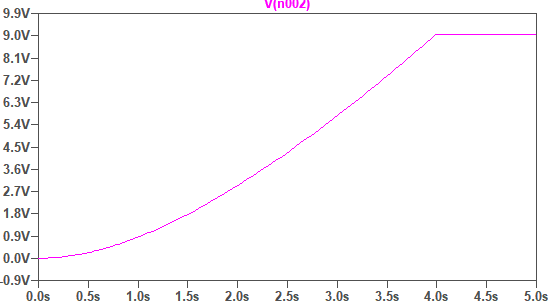
\includegraphics[width=12cm]{images/PD_pratico/OL.png}  
\end{center}
\caption{Simulação da planta em malha aberta(LTspice).}
\label{OL} 
\end{figure}

Podemos notar que ao passa do tempo o circuito saturará, pois como o LTspice trata os componentes da simulação de forma real logo não podemos aplicar valores infinitos de tensão na entrada.

Para planta em malha fechada, como pode ver no circuito do apêndice A.2, notamos que o comportamento como analisado anteriormente é oscilatório amortecido, devido o sistema ser estável, porém, não possuir um bom tempo de estabilização e um bom percentual de overshoot, com isso não temos uma boa MF. Nesse tipo de situação notamos evidentemente a necessidade de um controlador para ajustar a saída.  


\begin{figure}[H]
\begin{center}
    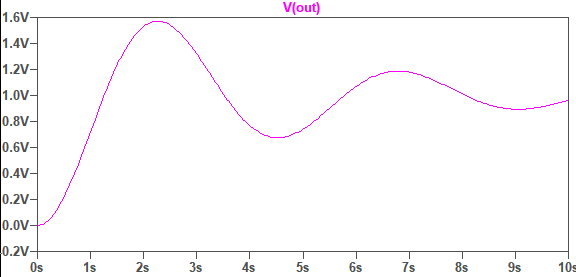
\includegraphics[width=12cm]{images/PD_pratico/CL.png}  
\end{center}
\caption{Simulação da planta em malha fechada(LTspice).}
\label{CL} 
\end{figure}

Agora analisando o circuito montado no LTspice  da planta em malha fechada mais o controlador PD, como pode ver no circuito do apêndice A.3, podemos notar um resultado bem melhor.  

\begin{figure}[H]
\begin{center}
    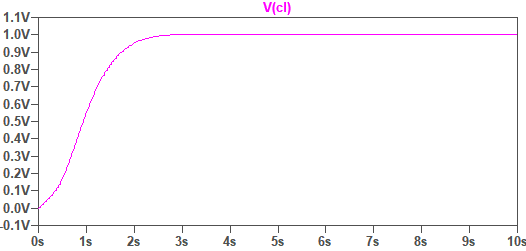
\includegraphics[width=12cm]{images/PD_pratico/NOVO_CL_PD.png}  
\end{center}
\caption{Simulação da planta em malha fechada em com PD(LTspice).}
\label{CL} 
\end{figure}

Podemos notar que no tempo, para os parâmetros estipulados e pela relação da margem de fase com o percentual de overshoot (equação \ref{mf}), um percentual abaixo dos obtemos um percentual em torno dos 5\%, além de tempo de estabilização muito bom, em torno dos 3 segundos.

\subsection{Resultados práticos}

Após a montagem do circuito utilizando AMPOPs do CI LM741, obteve-se uma série de formas de ondas. Vale destacar que: o canal 1 (CH1) do osciloscópio representa a saída do circuito; o canal 2 (CH2) representa a referência, que no caso é um degrau unitário; e o canal MATH representa a subtração entre a referência e a saída, ou seja, o erro.

O primeiro circuito implementado representou apenas a planta em malha aberta. Como observado na figura \ref{res:pd1}, ao inserir o degrau na entrada do circuito, o sistema instabilizou. Como se trata de um sistema prático, o valor de saída saturou no valor de alimentação dos AMPOPs, ao invés de tender a infinito. Pela mesma lógica o valor do erro também satura.


\begin{figure}[h!]
\begin{center}
    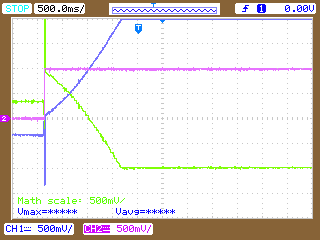
\includegraphics[width=10cm]{images/PD_pratico/ol1.png}  
\end{center}
\caption{Resultado prático da planta em malha aberta.}
\label{res:pd1} 
\end{figure}

O primeiro circuito implementado representou apenas a planta em malha fechada, ou seja, com o circuito da planta e do subtrator. Como observado na figura \ref{res:pd2}, ao inserir o degrau na entrada do circuito, a resposta oscilou bruscamente até tender ao valor de referência. Ao observar a escala de tensão, observa-se que o valor máximo de tensão para a saída é de 1.4V, com a entrada de 1V. Dessa forma o percentual de overshoot é de 28.57\%, resultando, pela equação \ref{mf}, em uma margem de fase de $37.04^{\circ}$.

\begin{figure}[h!]
\begin{center}
    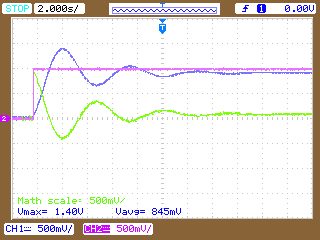
\includegraphics[width=10cm]{images/PD_pratico/cl1.png}  
\end{center}
\caption{Resultado prático da planta em malha fechada.}
\label{res:pd2} 
\end{figure}

O terceiro circuito implementado representou o sistema em malha fechada e com o controlador PD, contendo os circuitos da planta, controlador PD e subtrator. Como observado na figura \ref{res:pd3}, ao inserir o degrau na entrada do circuito, a resposta alcançou o valor de referência suavemente. Ao observar a escala de tensão, observa-se que o valor máximo de tensão para a saída é cerca de 1.04V (desprezando o ruído contido nas medições do osciloscópio e medindo com cursores) com a entrada de 1V. Dessa forma o percentual de overshoot é de 3.84\%, resultando, pela equação \ref{mf}, em uma margem de fase de $71.98^{\circ}$.

\begin{figure}[h!]
\begin{center}
    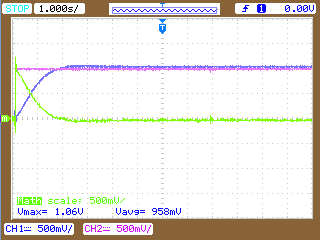
\includegraphics[width=10cm]{images/PD_pratico/c1.png}  
\end{center}
\caption{Resultado prático da planta em malha fechada e com PD.}
\label{res:pd3} 
\end{figure}

\pagebreak